\chapter{Experimental setup}
In this chapter we describe the setup we use for our experiments. All results of our experiments, as displayed in chapter \ref{ch:results}, are measured over a corpus of Java projects. In this chapter we will explain how we prepared this corpus.

\section{The corpus}\label{chap:corpus}
For our measurements we use a large corpus of open source projects \cite{githubCorpus2013}. This corpus has been assembled to contain relatively higher quality projects. Also, any duplicate projects were removed from this corpus. This results in a variety of Java projects that reflect the quality of average open source Java systems and are useful to perform measurements on.

As indicated in chapter \ref{chap:challenge} CloneRefactor requires all libraries of software projects we test. As these are not included in the used corpus \cite{githubCorpus2013}, we decided to filter the corpus to only include Maven projects. Maven is a build automation tool used primarily for Java, and works on basis of an \texttt{pom.xml} file to describe the projects' dependencies. As no \texttt{pom.xml} files are included in the corpus, we cloned the latest version of each project in the corpus. We then removed each project that has no \texttt{pom.xml} file. As a final step, we collected all dependencies for each project by using the \texttt{mvn dependency:copy-dependencies -DoutputDirectory=lib} Maven command, and removed each project for which not all dependencies were available (due to non-Maven dependencies being used or unsatisfiable dependencies being referenced in the \texttt{pom.xml} file).

Some general data regarding this corpus is displayed in Table \ref{table:general}.

\begin{table}[H]
  \begin{center}
  \caption{General results for GitHub Java projects corpus \cite{githubCorpus2013}.} \label{table:general}
  \medskip
\begin{tabular}{|l|l|}
\hline
Amount of projects                                                                                      & 1,361      \\ \hline
\begin{tabular}[c]{@{}l@{}}Amount of lines (excluding\\whitespace, comments and newlines.)\end{tabular} & 1,414,996  \\ \hline
Amount of statements/declarations                                                                       & 1,212,189  \\ \hline
\begin{tabular}[c]{@{}l@{}}Amount of tokens (excluding\\whitespace, comments and newlines.)\end{tabular} & 11,643,194 \\ \hline
\end{tabular}
\end{center}
\end{table}

\section{Context Analysis of Clones}\label{chap:contextsetup}
To be able to refactor code clones, it is important to consider the context of the clone. We define the following aspects of the clone as its context:
\begin{enumerate}
  \item \textbf{Relation:} The relation of clone instances among each other through inheritance.
  \item \textbf{Location:} Where a clone instance occurs in the code.
  \item \textbf{Contents:} The statements/declarations of a clone instance.
\end{enumerate}
We perform experiments on each of these aspects, defining categories and measuring these categories over the corpus.

\begin{figure}[H]
    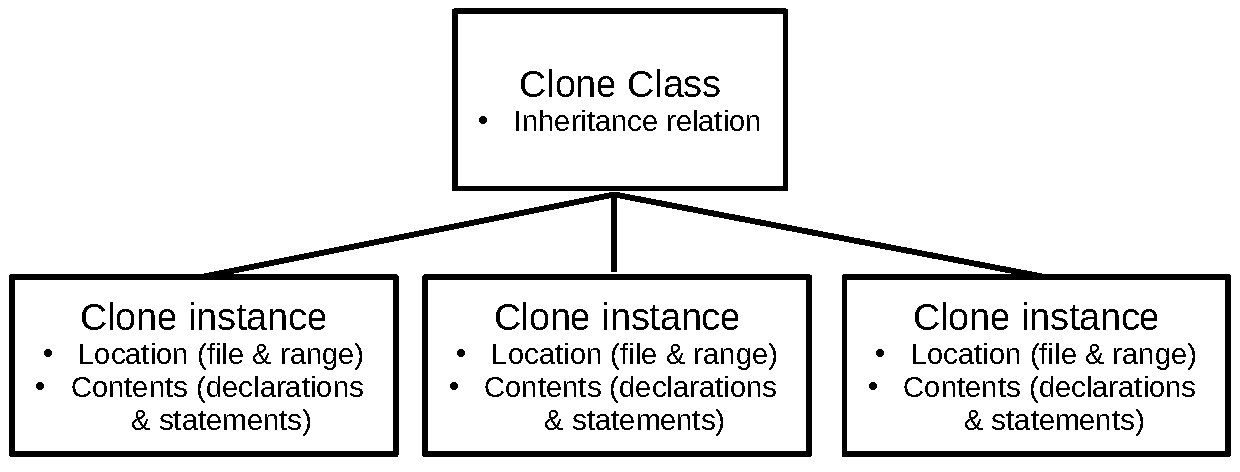
\includegraphics[width=0.6\columnwidth]{img/context}
    \caption{Abstract representation of clone classes and clone instances.}
  \label{fig:clonecontext}
\end{figure}

Fig.~\ref{fig:clonecontext} shows an abstract representation of clone classes and clone instances. The relation of clones through inheritance is measured for each clone class. The location and contents of clones are measured for each clone instance.

\subsection{Relation}\label{sec:setuprelationsinstances}
When merging code clones in object-oriented languages, it is important to consider the inheritance relation between clone instances. This relation has a big impact on how a clone should be refactored.

Fontana et al.~\cite{fontana2015duplicated} describe measurements on 50 open source projects on the relation of clone instances to each other. To do this, they first define several categories for the relation between clone instances in object-oriented languages. These categories are as follows:
\begin{enumerate}
  \item \textbf{Same Method}: All instances of the clone class are in the same method.
  \item \textbf{Same Class}: All instances of the clone class are in the same class.
  \item \textbf{Superclass}: All instances of the clone class are in a class that is child or parent of each other.
  \item \textbf{Ancestor Class}: All instances of the clone class are superclasses except for the direct superclass.
  \item \textbf{Sibling Class}: All instances of the clone class have the same parent class.
  \item \textbf{First Cousin Class}: All instances of the clone class have the same grandparent class.
\item \textbf{Same Hierarchy Class}: All instances of the clone class belong to the same inheritance hierarchy, but do not belong to any of the other categories.
\item \textbf{Same External Superclass}: All instances of the clone class have the same superclass, but this superclass is not included in the project but part of a library.
\item \textbf{Unrelated class}: There is at least one instance in the clone class that is not in the same hierarchy.
\end{enumerate}

We added the following categories, to gain more information about clones and reduce the number of unrelated clones:

\begin{enumerate}
\item \textbf{Same Interface}: All instances of the clone class are in a class or interface that have a common interface anywhere in their inheritance hierarchy.
\item \textbf{No Direct Superclass}: All instances of the clone class are in a class that does not have any superclass.
\item \textbf{No Indirect Superclass}: All instances of the clone class are in a class that does not have any external classes in its inheritance hierarchy.
\end{enumerate}

Figure \ref{fig:clonecontext} shows an abstract representation of clone classes and clone instances. The relation of clones through inheritance is measured on clone class level: it involves all child clone instances. The location and contents of clones is measured on clone instance level. A clone's location involves the file it resides in and the range it spans (for example: line 6 col 2 - line 7 col 50). A clone instance contents consists of a list of all statements and declarations it spans.

\begin{figure}[H]
  \caption{Abstract figure displaying relations of clone classes. Arrows represent superclass relations.}
    \medskip
    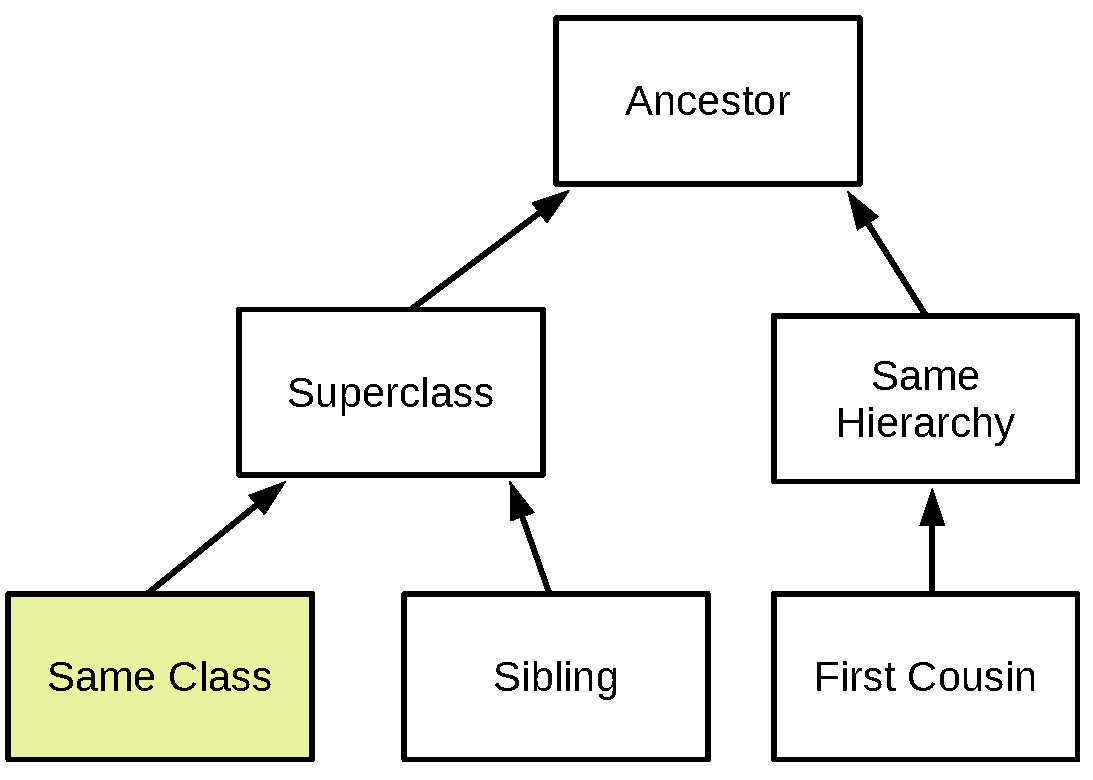
\includegraphics[width=1\columnwidth]{img/Relation}
  \label{fig:clonerelation}
\end{figure}

We separate these relations into the following categories, because of their related refactoring opportunities:
\begin{itemize}
  \item \textbf{Common Class}: \textit{Same Method}, \textit{Same Class}
  \item \textbf{Common Hierarchy}: \textit{Superclass}, \textit{Ancestor Class}, \textit{Sibling Class}, \textit{First Cousin}, \textit{Same Hierarchy}
  \item \textbf{Common Interface}: \textit{Same Interface}
  \item \textbf{Effectively Unrelated}: \textit{No Direct Superclass}, \textit{No Indirect Superclass}, \textit{External Superclass}, \textit{Unrelated}
\end{itemize}

Every clone class only has a single relation, which is the first relation from above list that the clone class applies to. For instance: all ``Superclass'' clones also apply to ``Same Hierarchy'', but because ``Superclass'' is earlier in above list they will get the ``Superclass'' relation. This is because the items earlier in the list denote a more favorable refactoring.

\subsubsection{Common Class}
The \textit{``Same method''} and \textit{``Same class''} relations share a common refactoring opportunity. Clones of both these catagories, when extracted to a new method, can be placed in the same class. Both of these relations are most favorable for refactoring, as they require a minimal design tradeoff. Furthermore, global variables that are used in the class can be used without having to create method parameters.

A clone class is flagged as ``Same method'' if all clone instances in the clone class are in the same method:

\begin{equation}\label{eq:samemethod}
\forall (i_1 \in C) \forall (i_2 in C) Mi_1 = Mi_2
\end{equation}

Where \textit{M} is the method in which a clone instance is found. Please note that a clone instance may not always be in a method, for which this predicate will fail. Each node in a clone instance is checked for this predicate, so if a single node of a clone instance is outside a method, the predicate will fail.

A clone class is flagged as ``Same class'' if all clone instances in the clone class are in the same class:

\begin{equation}\label{eq:samemethod}
\forall (i_1 \in C) \forall (i_2 in C) Di_1 = Di_2
\end{equation}

Where \textit{D} is the class declaration in which the clone instance is found.

\subsubsection{Common Hierarchy}
The following relations belong to
\todo{TODO}

\subsubsection{Common Interface}
\todo{TODO}

\subsubsection{Effectively Unrelated}
\todo{TODO}
